This section includes information on previously presented \href{https://indico.bnl.gov/event/25153/contributions/97868/attachments/57967/99541/10.16.24.pdf}{initial studies of this analysis} that found the reconstructed \ET{} to be highly dependent on the reconstruction method and noise contributions while the \ET{} from topoclusters is much less dependent on the reconstruction method and noise level. 

Four Monte Carlo datasets were used to compare to data in the initial studies of this analysis. The first three datasets were all using the default sPHENIX Pythia8 generator "jet 10" dataset which has a simulation trigger requirement of 10 GeV jets. The three datasets differed in their calorimeter reconstruction methodology. The first is "calo cluster" which was the previous default MC calorimeter reconstruction method, here the calibrated energy comes directly from g4hits (no waveform fitting); there is a 1 ADC width noise in digitization step for all calorimeters, a 30 MeV tower energy threshold in EMCal and 0 MeV tower energy threshold in HCals. The second is calo nozero" where the calibrated energy also comes from from g4hits (no waveform fitting); there is a  1 ADC width noise in digitization step but no tower energy threshold for all calorimeters. The final is "calo waveform" which uses a waveform fitting/processing module to calibrate energy from g4hits, has realistic tower-by-tower noise, and hardware style ZS but with uniform (not tower-by-tower) ZS thresholds.
The final monte carlo dataset that is used in the initial studies is the detroit Pythia8 tune "jet 10" dataset coupled with the "calo waveform" reconstruction method. 

\subsection{Jet QA}
Initial data to monte carlo comparisons of dijet variables include the following: spectra of leading + subleading jet pT, dijet $\delta\phi$ distribution, and dijet asymmetry $x_{j}$ shown in Fig. \ref{fig:dijet_qa}. 

\begin{figure}
    \centering
    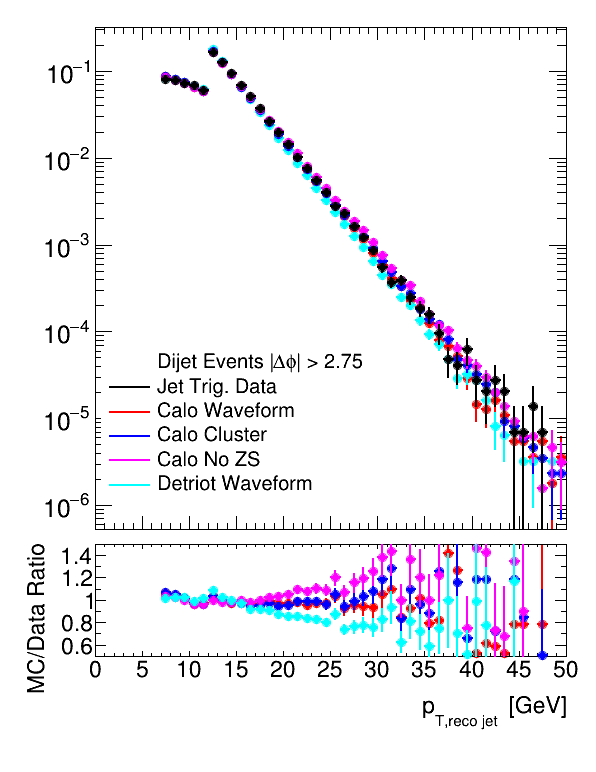
\includegraphics[width=0.32\linewidth]{Figures/initial_studies/h_jetspectra.png}
    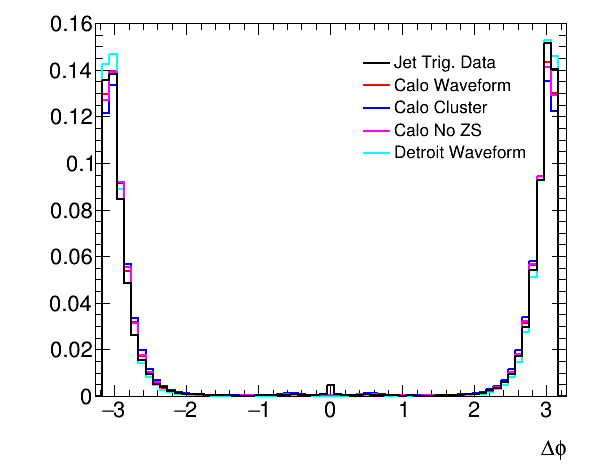
\includegraphics[width=0.32\linewidth]{Figures/initial_studies/h_deltaphi.png}
    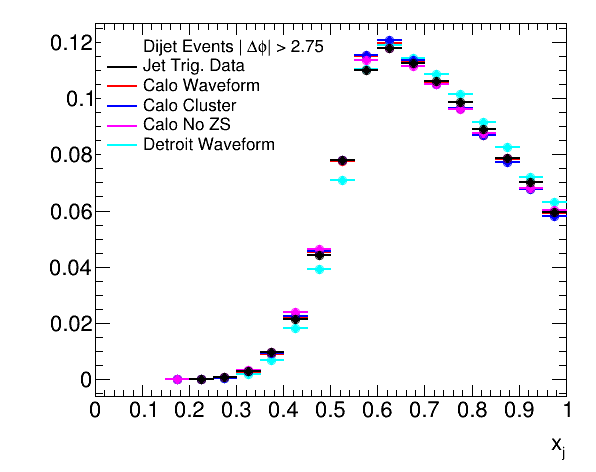
\includegraphics[width=0.32\linewidth]{Figures/initial_studies/h_xj.png}
    \caption{Data to MC comparison of leading + subleading jet pT (left), dijet $\delta\phi$ (center) and dijet asymmetry (right) in dijet events using ana430p007 data, Run 15 calo waveform, nozero and cluster, and Run 150 (detroit) waveform.}
    \label{fig:dijet_qa}
\end{figure}

\subsection{Topocluster reconstruction}
Topoclusters are reconstructed using the default topoclustering module found in the G4\_TopoClusterReco.C macro. Topoclusters are created using all three layers of the calorimeters. The default topoclustering parameters are as follows: 
\begin{verbatim}
  RawClusterBuilderTopo* ClusterBuilder = new 
            RawClusterBuilderTopo("HcalRawClusterBuilderTopo");
  ClusterBuilder->Verbosity(verbosity);
  ClusterBuilder->set_nodename("TOPOCLUSTER_ALLCALO");
  ClusterBuilder->set_enable_HCal(true);
  ClusterBuilder->set_enable_EMCal(true);
  ClusterBuilder->set_noise(0.0025, 0.006, 0.03);
  ClusterBuilder->set_significance(4.0, 2.0, 0.0);
  ClusterBuilder->allow_corner_neighbor(true);
  ClusterBuilder->set_do_split(true);
  ClusterBuilder->set_minE_local_max(1.0, 2.0, 0.5);
  ClusterBuilder->set_R_shower(0.025);
  ClusterBuilder->set_use_only_good_towers(true);
  ClusterBuilder->set_absE(true);
  se->registerSubsystem(ClusterBuilder);  
\end{verbatim}

\subsection{UE from towers versus topoclusters}
Initial studies of the reconstructed transverse energy in dijet events compared the energy density from summing calorimeter towers versus the energy density from summing topoclusters. A comparison of the sum energy density distributions in the towards, transverse and away regions of dijet events is presented in Fig. \ref{fig:towers_vs_topo}. The \ET from towers is highly dependent on the reconstruction method and noise contributions while the \ET from topoclusters is much less dependent on the reconstruction method and noise level. 

\begin{figure}
    \centering
    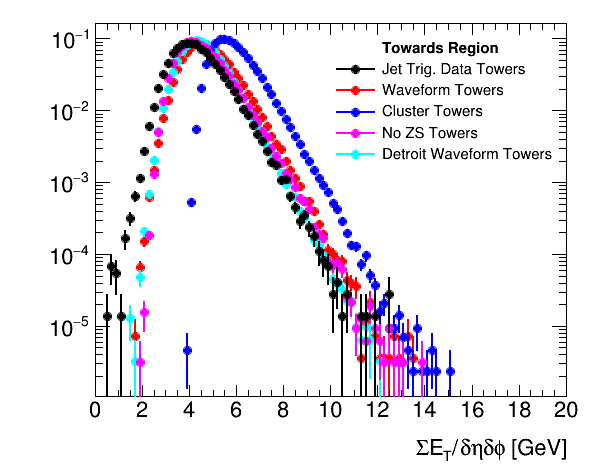
\includegraphics[width=0.32\linewidth]{Figures/initial_studies/h_ue_towards_towers.png}
    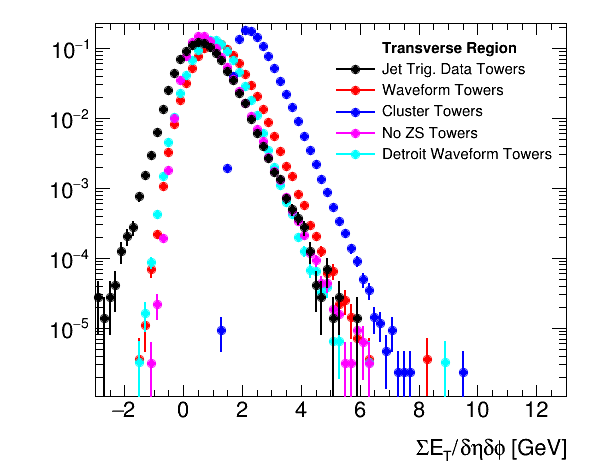
\includegraphics[width=0.32\linewidth]{Figures/initial_studies/h_ue_transverse_towers.png}
    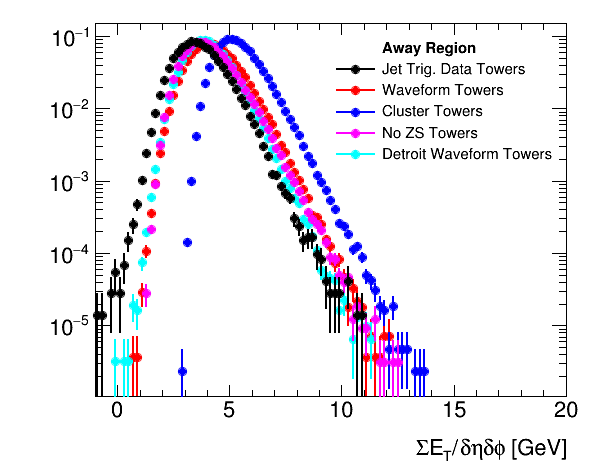
\includegraphics[width=0.32\linewidth]{Figures/initial_studies/h_ue_away_towers.png}
    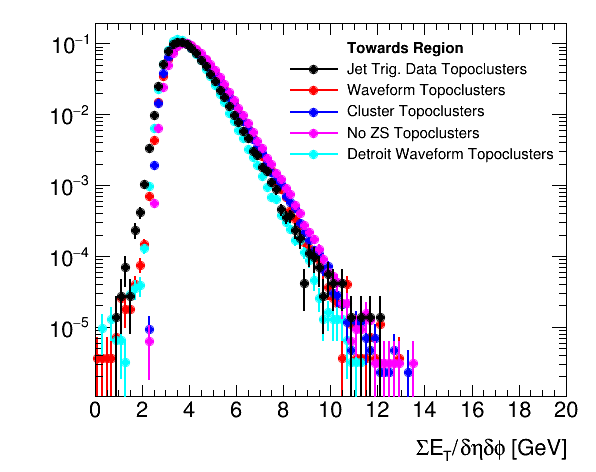
\includegraphics[width=0.32\linewidth]{Figures/initial_studies/h_ue_towards_topoclusters.png}
    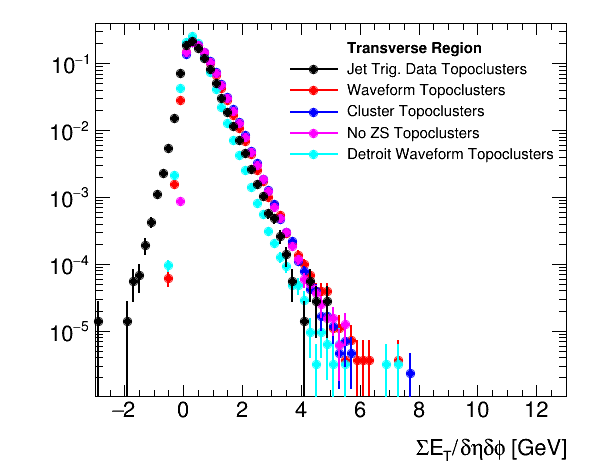
\includegraphics[width=0.32\linewidth]{Figures/initial_studies/h_ue_transverse_topoclusters.png}
    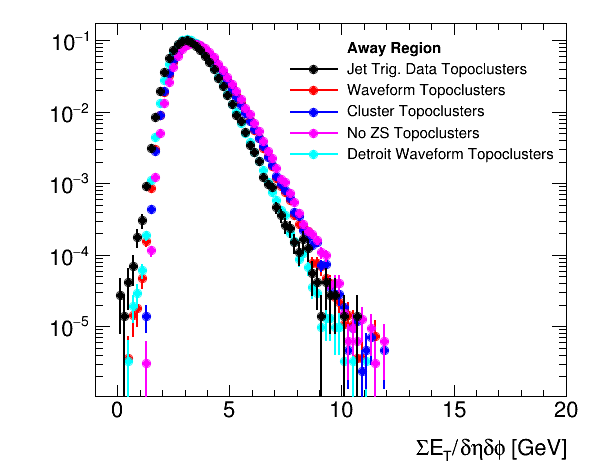
\includegraphics[width=0.32\linewidth]{Figures/initial_studies/h_ue_away_topoclusters.png}
    \caption{Comparison of topocluster transverse energy distributions in dijet events using ana430p007 data, Run 15 calo waveform, nozero and cluster, and Run 150 (Detroit) waveform. No energy threshold applied to topocluster energy sum.}
    \label{fig:towers_vs_topo}
\end{figure}

\subsection{UE from Topoclusters QA}
Further efforts to compare the UE from topoclusters in data versus monte carlo were looked at by looking at the number of topoclusters in each of the three dijet regions, towards, transverse and away, as well as the topocluster transverse energy spectra in each of these regions. To understand influences from noise and waveform reconstruction on the topoclusters formed in data and monte carlo, 6 energy thresholds on the topoclusters included in the number of topoclusters distribution and topocluster transverse energy spectrum were investigated. These energy thresholds were as follows: all topoclusters (no $E_{topo}$ cut), $E_{topo} >$ 0, $E_{topo} >$ 100 MeV, $E_{topo} >$ 200 MeV, $E_{topo} >$ 300 MeV and $E_{topo} >$ 500 MeV. Fig. \ref{fig:ntopo_etopo_means} shows a data to monte carlo comparison of the mean and width of the number of topoclusters distribution and topocluster transverse energy spectrum as a function of $E_{topo}$ threshold. 

\begin{figure}
    \centering
    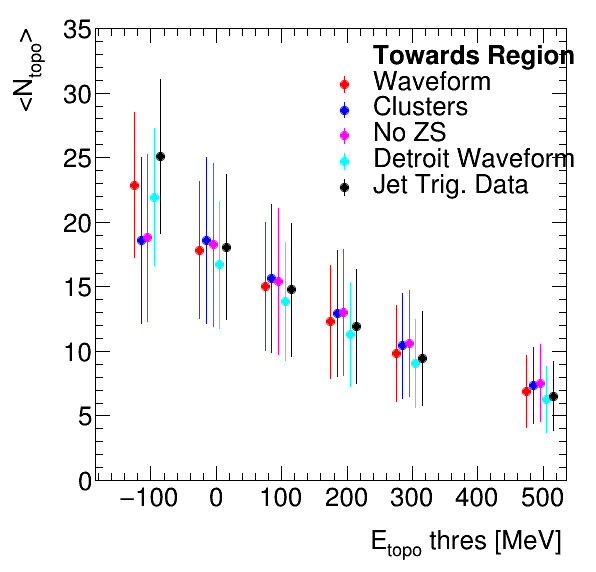
\includegraphics[width=0.32\linewidth]{Figures/initial_studies/h_mean_ntopo_towards.png}
    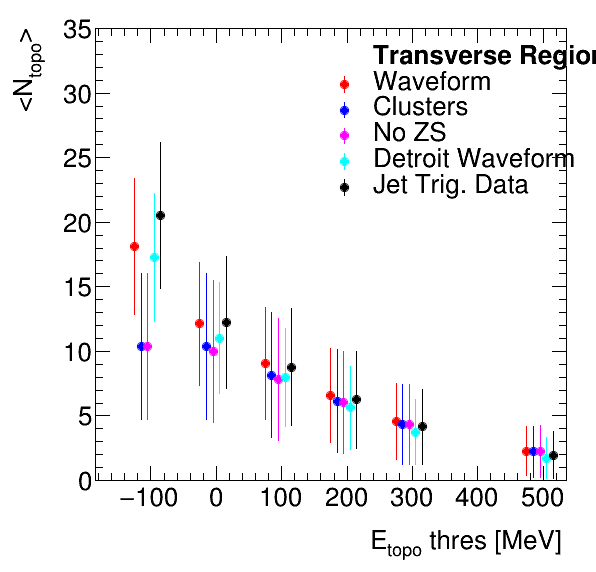
\includegraphics[width=0.32\linewidth]{Figures/initial_studies/h_mean_ntopo_transverse.png}
    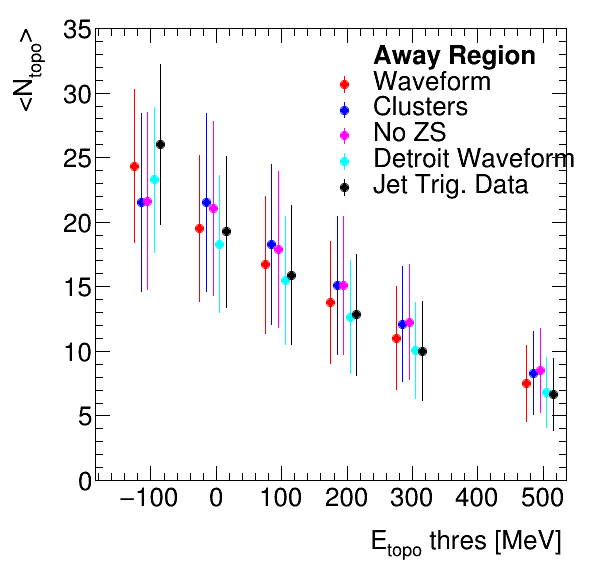
\includegraphics[width=0.32\linewidth]{Figures/initial_studies/h_mean_ntopo_away.png}
    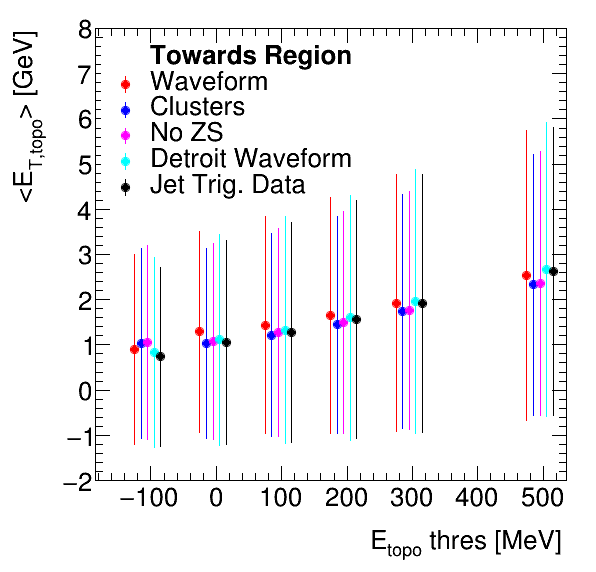
\includegraphics[width=0.32\linewidth]{Figures/initial_studies/h_mean_etopo_towards.png}
    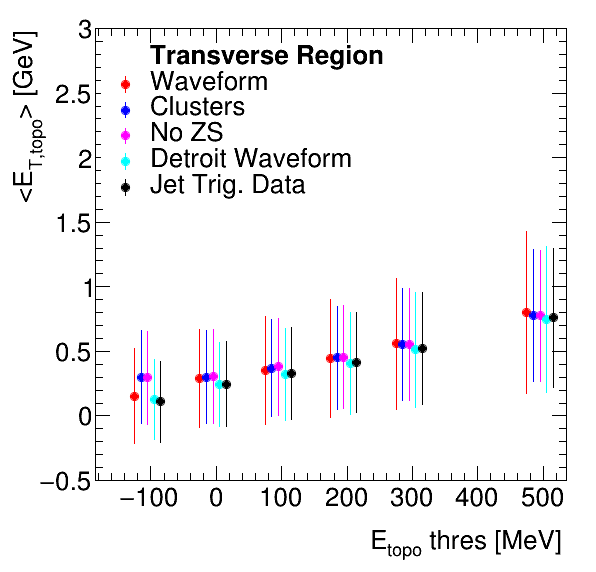
\includegraphics[width=0.32\linewidth]{Figures/initial_studies/h_mean_etopo_transverse.png}
    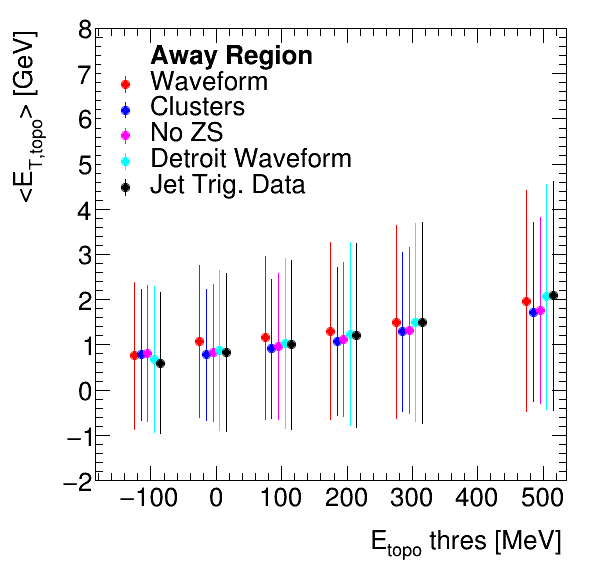
\includegraphics[width=0.32\linewidth]{Figures/initial_studies/h_mean_etopo_away.png}
    \caption{Mean number of topoclusters (upper plots) and topocluster transverse energy spectrum (lower plots) in the towards (right), transverse (center) and away (right) regions. Comparison of topoclusters in dijet events using ana430p007 data, Run 15 calo waveform, nozero and cluster, and Run 150 (Detroit) waveform. Note error bars here represent the distribution width.}
    \label{fig:ntopo_etopo_means}
\end{figure}

The full number of topocluster distributions and topocluster transverse energy spectra are included in Figs.~\labelcref{fig:ntopo_towards,fig:ntopo_transverse,fig:ntopo_away,fig:topo_spectra_towards,fig:topo_spectra_transverse,fig:topo_spectra_away}. With the inclusion of even a $E_{topo} > 0$ MeV threshold, we see good agreement between data and monte carlo for nearly all reconstruction methods. Two notable comparisons are that the detroit waveform and default pythia waveform datasets reconstruct the topocluster number and energy spectra best in comparison to data in the regions of a hard scattering (towards and away) and that only the detroit waveform dataset agrees with the data topocluster energy spectra in the transverse region. 

\begin{figure}
    \centering
    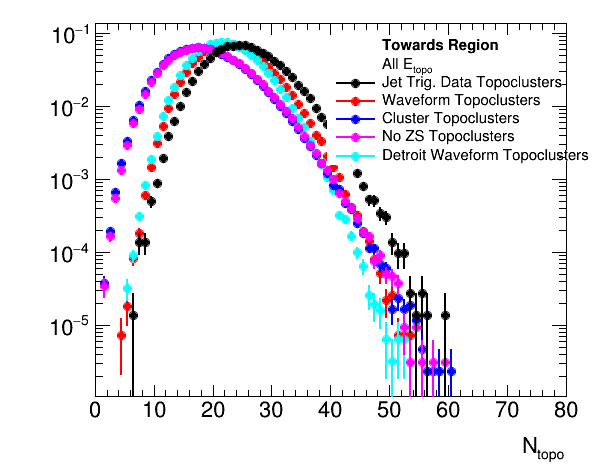
\includegraphics[width=0.32\linewidth]{Figures/initial_studies/h_ntopo_towards-9999_Topoclusters.png}
    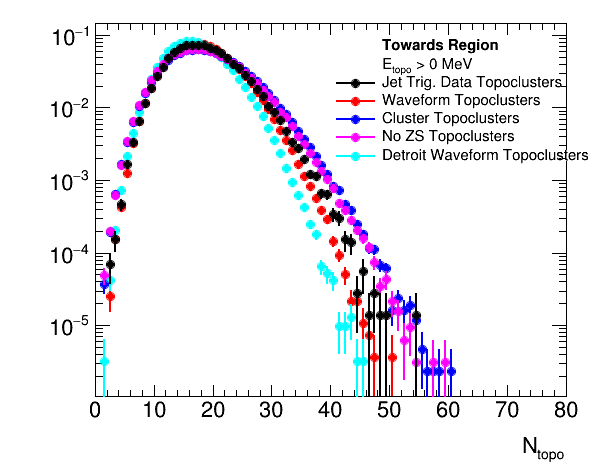
\includegraphics[width=0.32\linewidth]{Figures/initial_studies/h_ntopo_towards0_Topoclusters.png}
    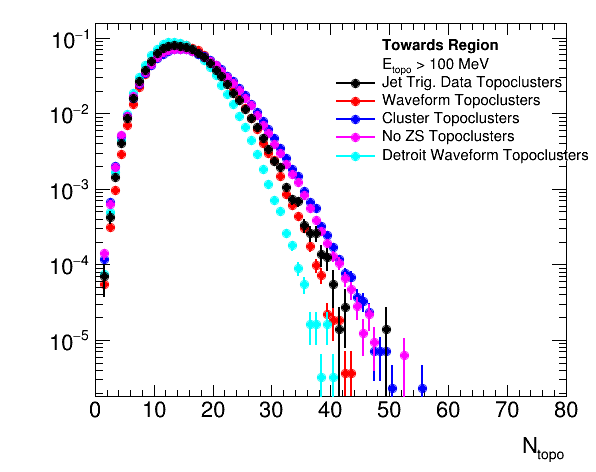
\includegraphics[width=0.32\linewidth]{Figures/initial_studies/h_ntopo_towards100_Topoclusters.png}
    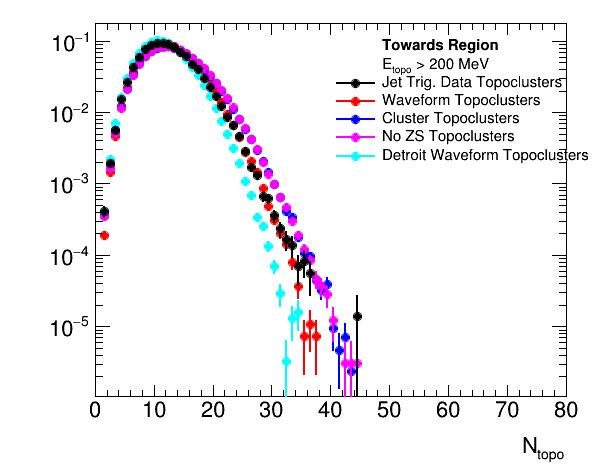
\includegraphics[width=0.32\linewidth]{Figures/initial_studies/h_ntopo_towards200_Topoclusters.png}
    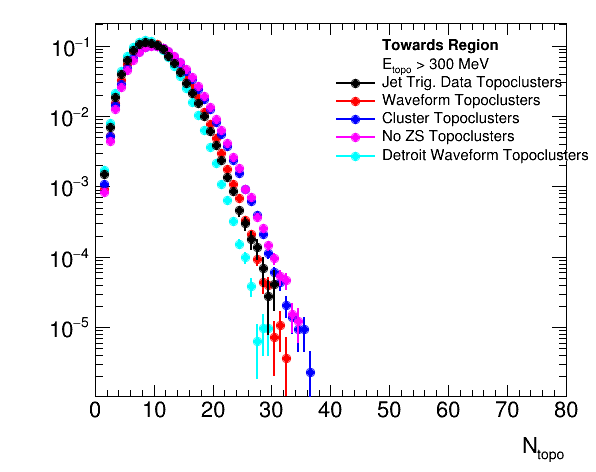
\includegraphics[width=0.32\linewidth]{Figures/initial_studies/h_ntopo_towards300_Topoclusters.png}
    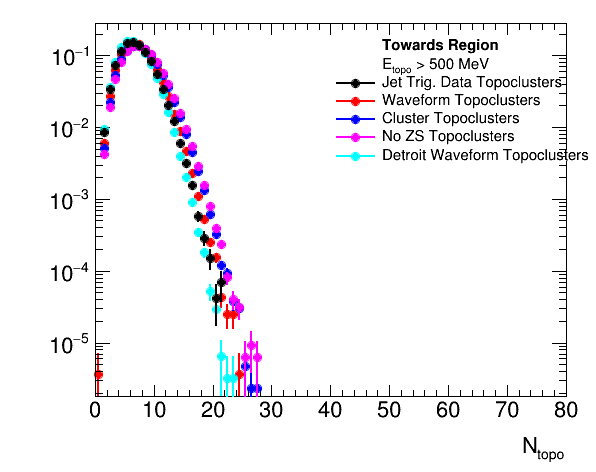
\includegraphics[width=0.32\linewidth]{Figures/initial_studies/h_ntopo_towards500_Topoclusters.png}
    \caption{Number of topoclusters in the towards region of dijet events for various $E_{topo}$ thresholds using ana430p007 data, Run 15 calo waveform, nozero and cluster, and Run 150 (Detroit) waveform jet 10 datasets.}
    \label{fig:ntopo_towards}
\end{figure}

\begin{figure}
    \centering
    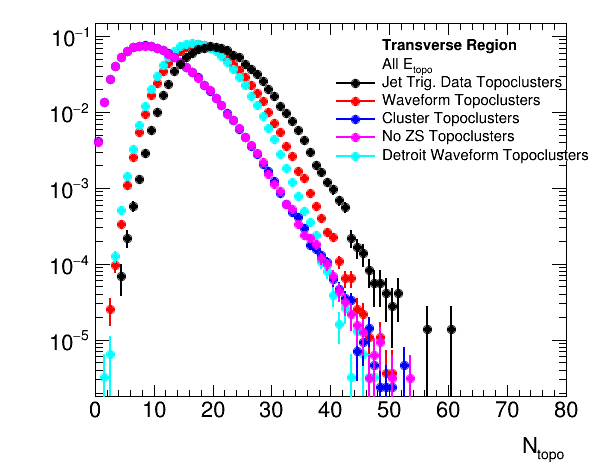
\includegraphics[width=0.32\linewidth]{Figures/initial_studies/h_ntopo_transverse-9999_Topoclusters.png}
    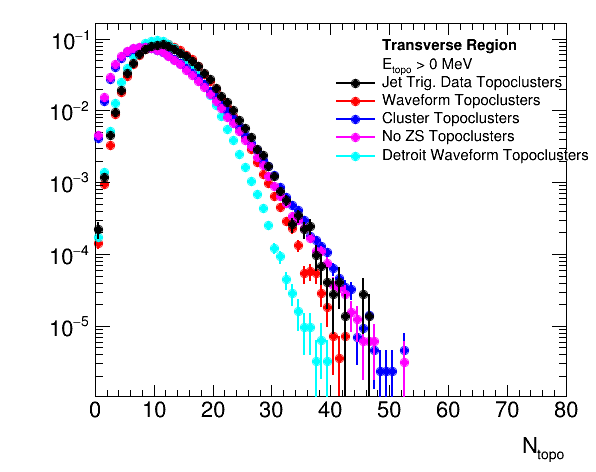
\includegraphics[width=0.32\linewidth]{Figures/initial_studies/h_ntopo_transverse0_Topoclusters.png}
    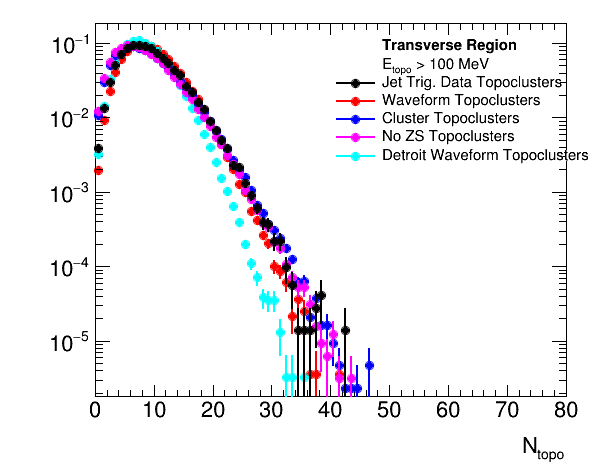
\includegraphics[width=0.32\linewidth]{Figures/initial_studies/h_ntopo_transverse100_Topoclusters.png}
    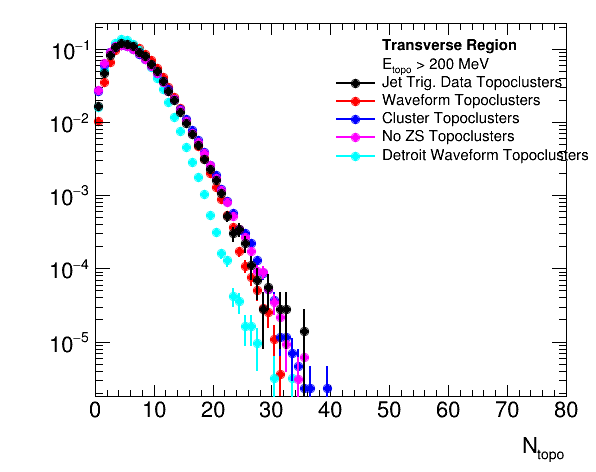
\includegraphics[width=0.32\linewidth]{Figures/initial_studies/h_ntopo_transverse200_Topoclusters.png}
    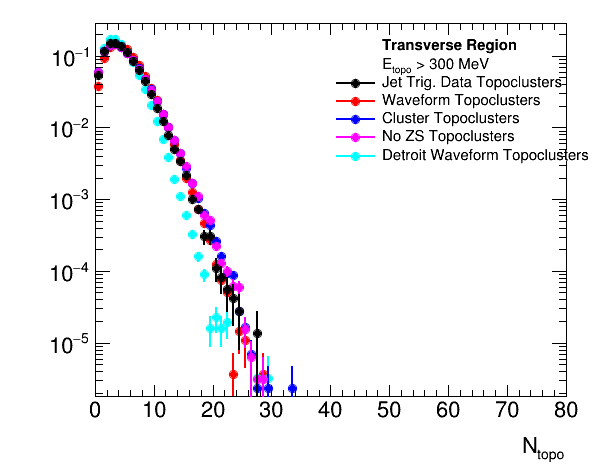
\includegraphics[width=0.32\linewidth]{Figures/initial_studies/h_ntopo_transverse300_Topoclusters.png}
    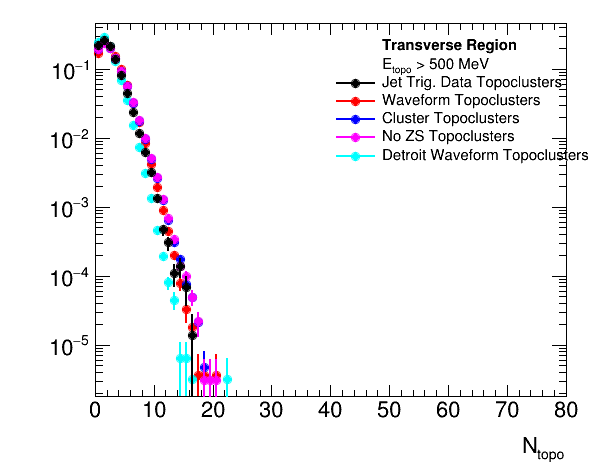
\includegraphics[width=0.32\linewidth]{Figures/initial_studies/h_ntopo_transverse500_Topoclusters.png}
    \caption{Number of topoclusters in the transverse region of dijet events for various $E_{topo}$ thresholds using ana430p007 data, Run 15 calo waveform, nozero and cluster, and Run 150 (Detroit) waveform jet 10 datasets.}
    \label{fig:ntopo_transverse}
\end{figure}

\begin{figure}
    \centering
    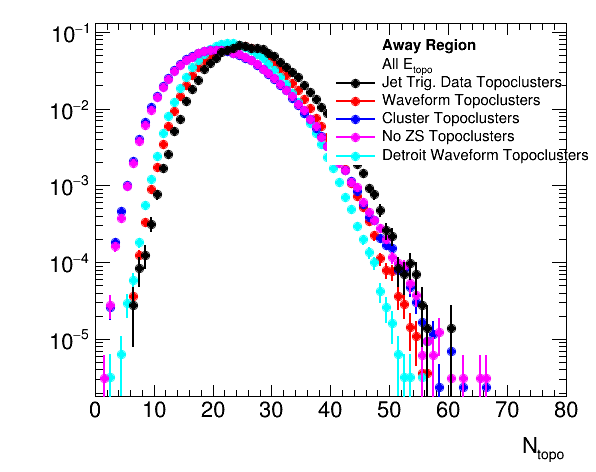
\includegraphics[width=0.32\linewidth]{Figures/initial_studies/h_ntopo_away-9999_Topoclusters.png}
    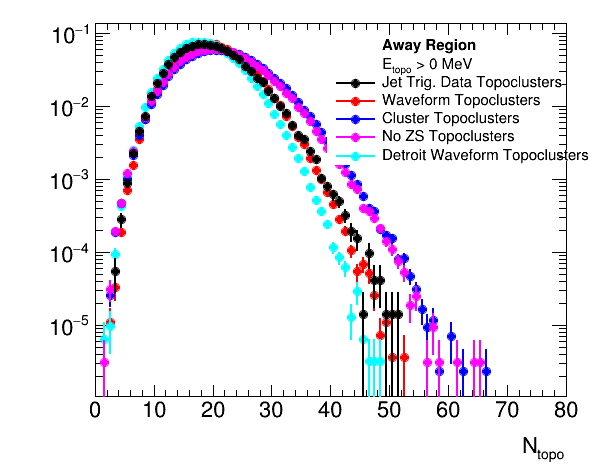
\includegraphics[width=0.32\linewidth]{Figures/initial_studies/h_ntopo_away0_Topoclusters.png}
    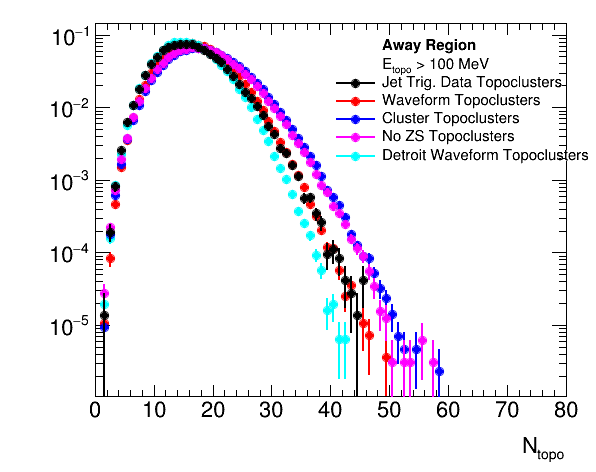
\includegraphics[width=0.32\linewidth]{Figures/initial_studies/h_ntopo_away100_Topoclusters.png}
    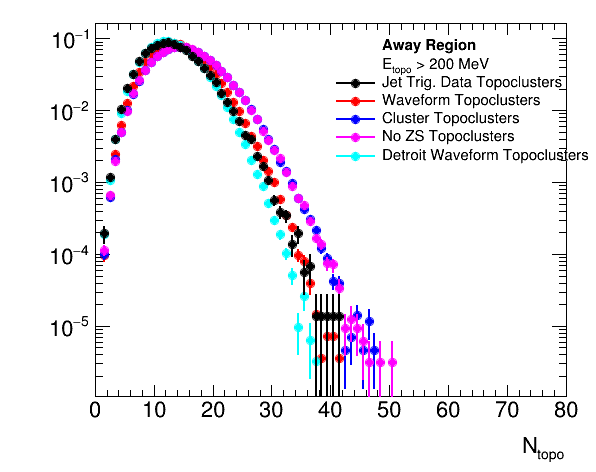
\includegraphics[width=0.32\linewidth]{Figures/initial_studies/h_ntopo_away200_Topoclusters.png}
    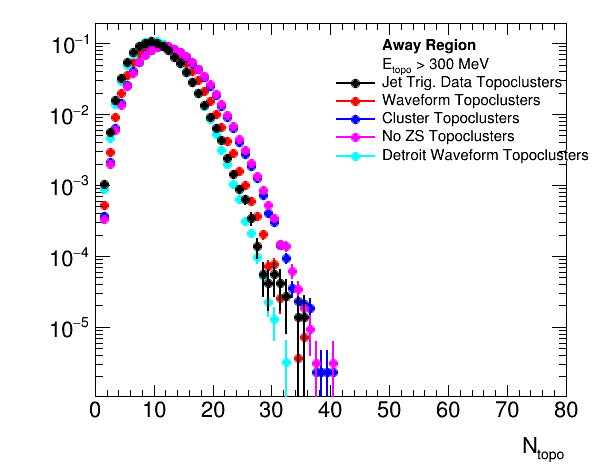
\includegraphics[width=0.32\linewidth]{Figures/initial_studies/h_ntopo_away300_Topoclusters.png}
    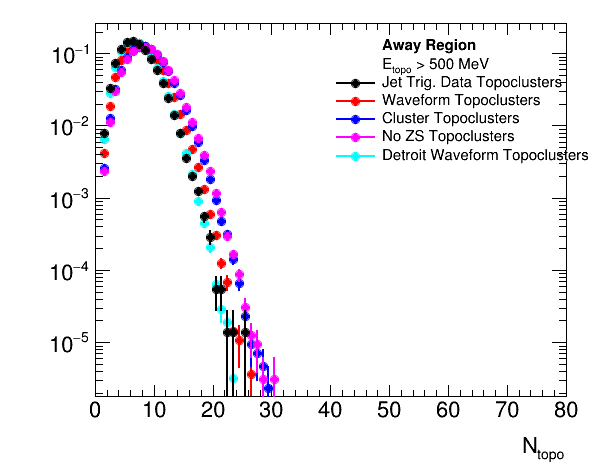
\includegraphics[width=0.32\linewidth]{Figures/initial_studies/h_ntopo_away500_Topoclusters.png}
    \caption{Number of topoclusters in the away region of dijet events for various $E_{topo}$ thresholds using ana430p007 data, Run 15 calo waveform, nozero and cluster, and Run 150 (Detroit) waveform jet 10 datasets.}
    \label{fig:ntopo_away}
\end{figure}

\begin{figure}
    \centering
    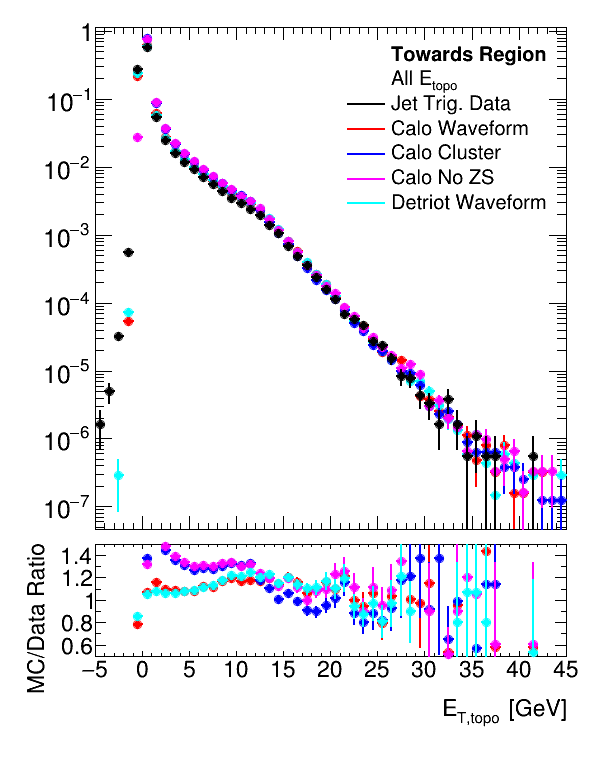
\includegraphics[width=0.32\linewidth]{Figures/initial_studies/h_topo_spectra_towards-9999_Topoclusters.png}
    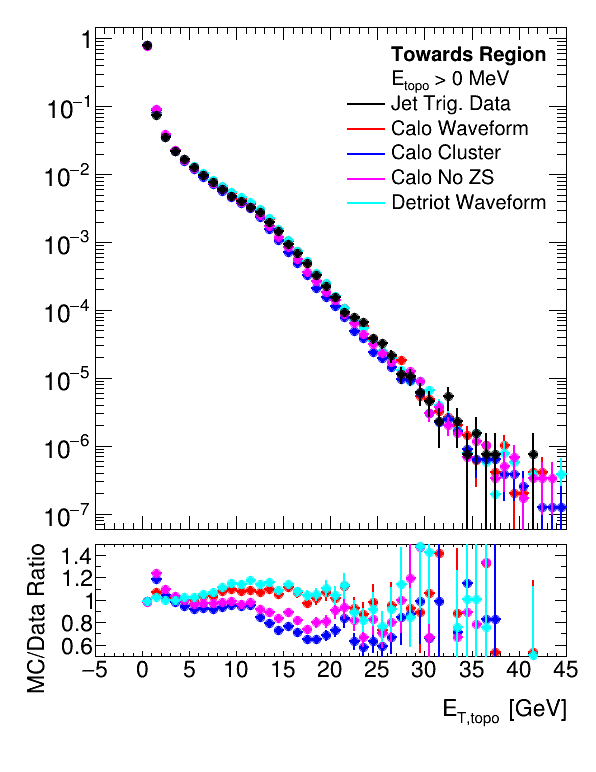
\includegraphics[width=0.32\linewidth]{Figures/initial_studies/h_topo_spectra_towards0_Topoclusters.png}
    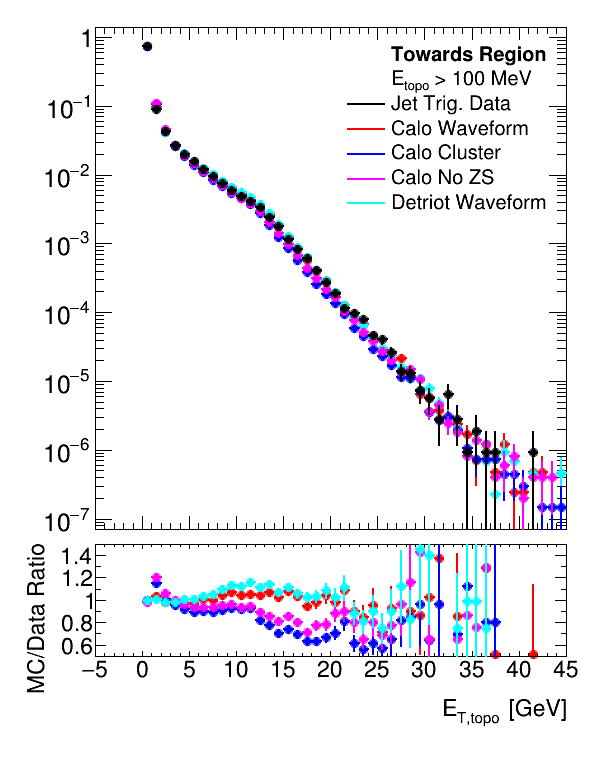
\includegraphics[width=0.32\linewidth]{Figures/initial_studies/h_topo_spectra_towards100_Topoclusters.png}
    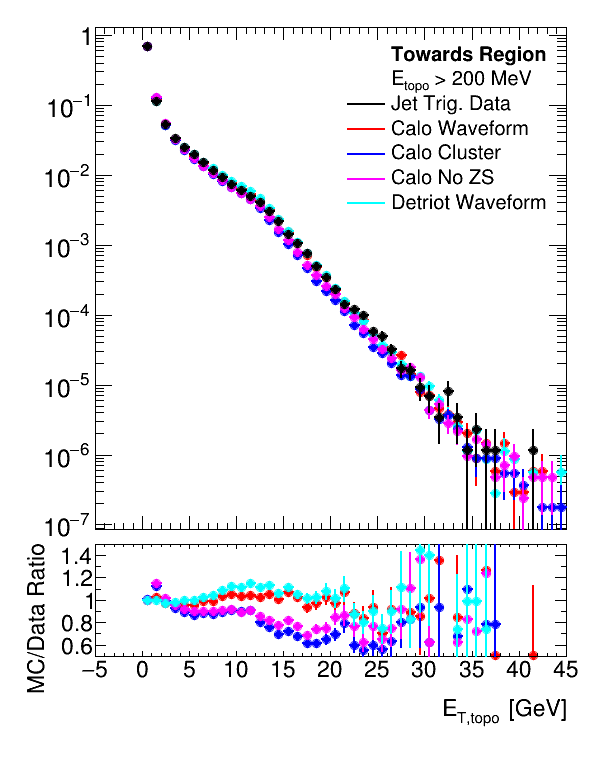
\includegraphics[width=0.32\linewidth]{Figures/initial_studies/h_topo_spectra_towards200_Topoclusters.png}
    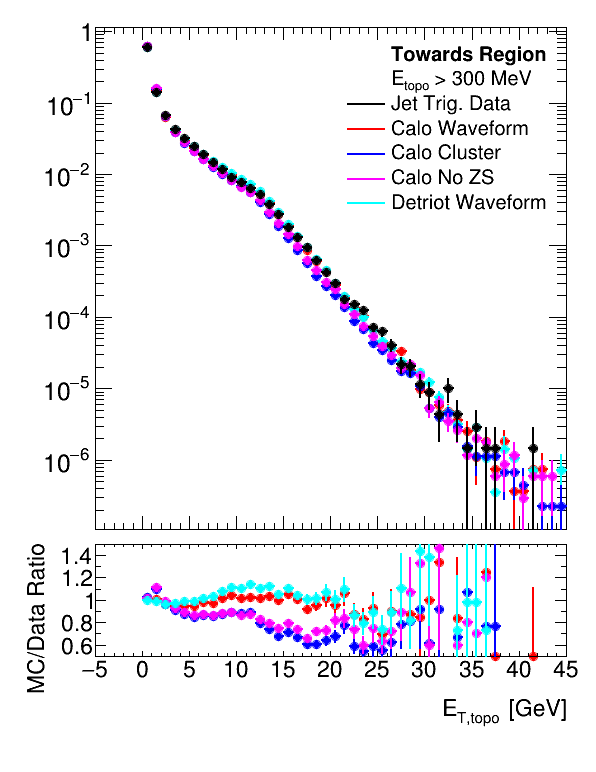
\includegraphics[width=0.32\linewidth]{Figures/initial_studies/h_topo_spectra_towards300_Topoclusters.png}
    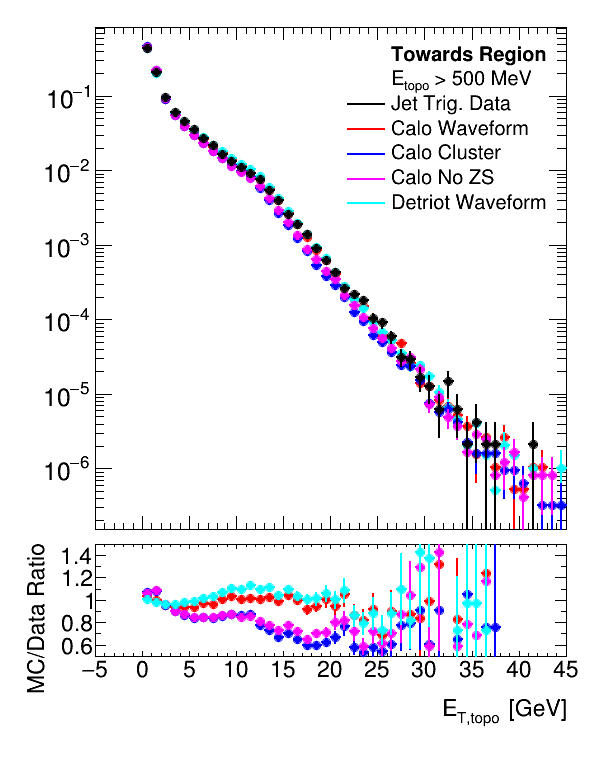
\includegraphics[width=0.32\linewidth]{Figures/initial_studies/h_topo_spectra_towards500_Topoclusters.png}
    \caption{Topocluster transverse energy spectra in the towards region of dijet events for various $E_{topo}$ thresholds using ana430p007 data, Run 15 calo waveform, nozero and cluster, and Run 150 (Detroit) waveform jet 10 datasets.}
    \label{fig:topo_spectra_towards}
\end{figure}

\begin{figure}
    \centering
    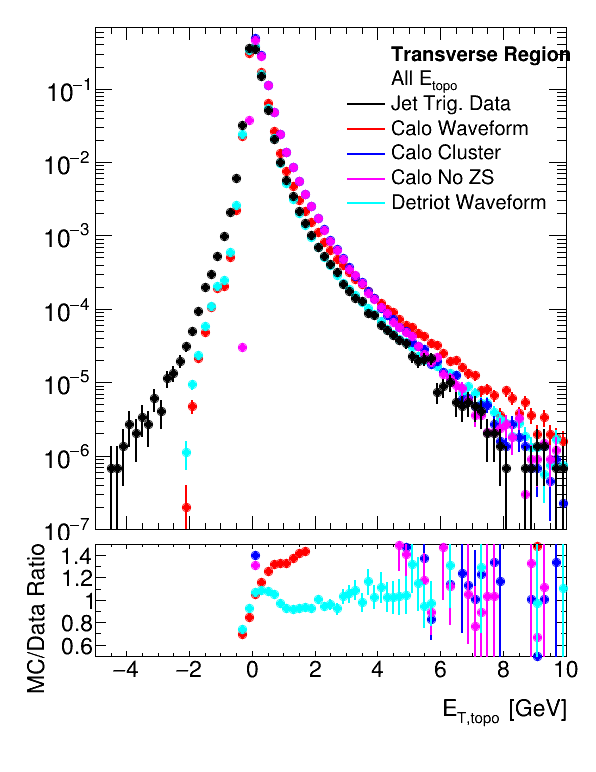
\includegraphics[width=0.32\linewidth]{Figures/initial_studies/h_topo_spectra_transverse-9999_Topoclusters.png}
    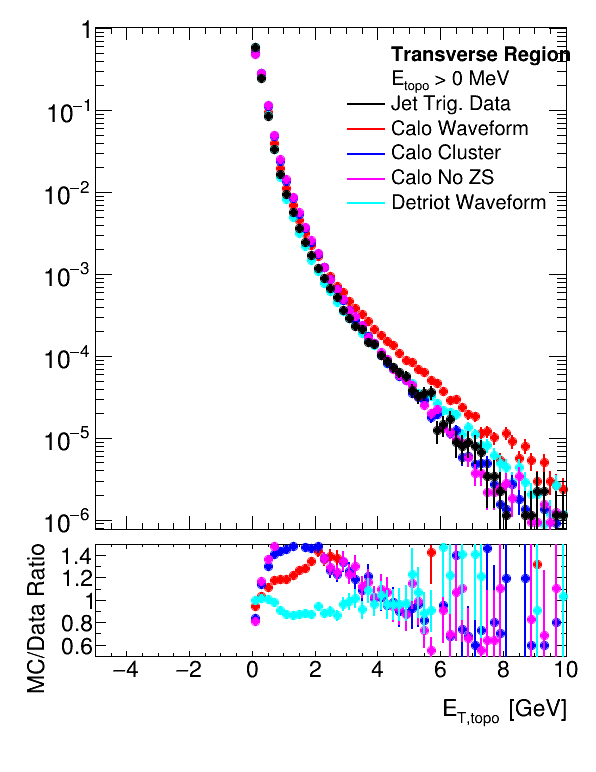
\includegraphics[width=0.32\linewidth]{Figures/initial_studies/h_topo_spectra_transverse0_Topoclusters.png}
    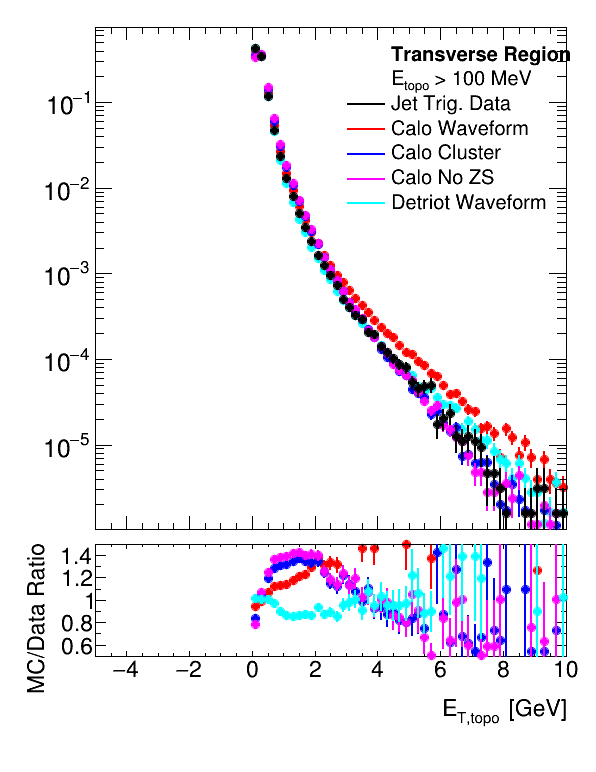
\includegraphics[width=0.32\linewidth]{Figures/initial_studies/h_topo_spectra_transverse100_Topoclusters.png}
    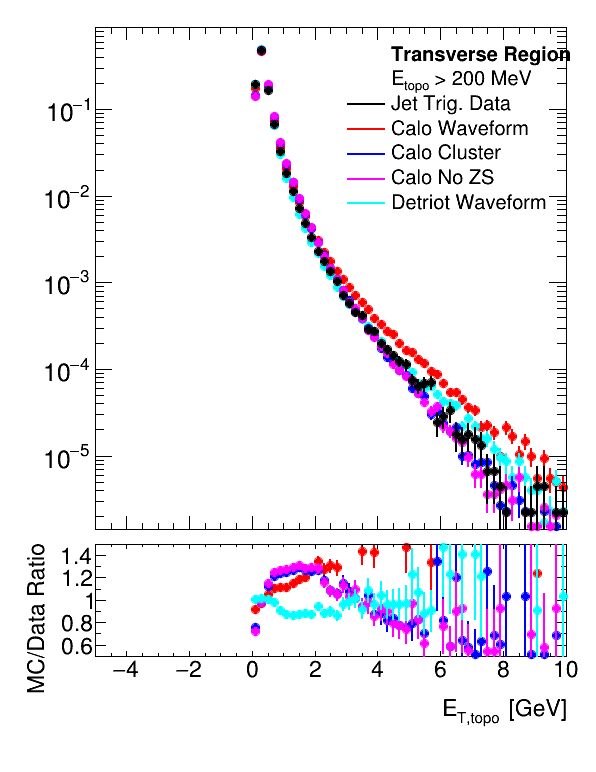
\includegraphics[width=0.32\linewidth]{Figures/initial_studies/h_topo_spectra_transverse200_Topoclusters.png}
    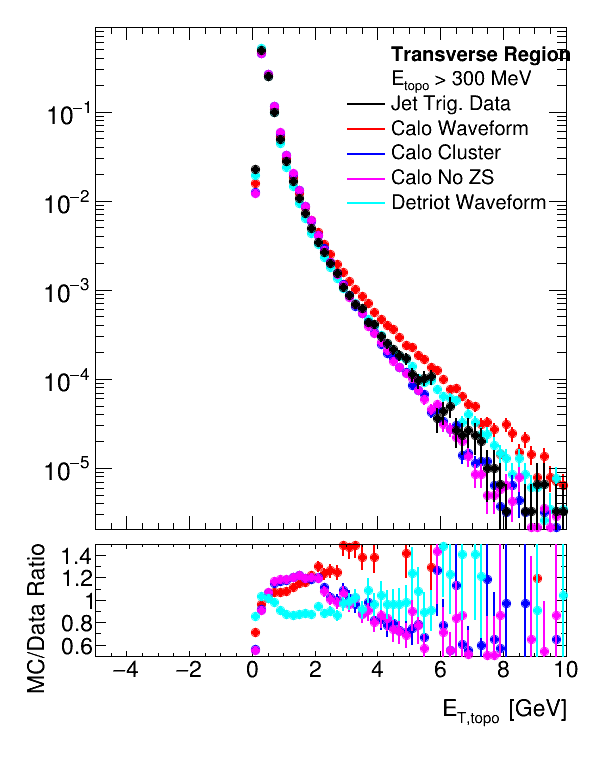
\includegraphics[width=0.32\linewidth]{Figures/initial_studies/h_topo_spectra_transverse300_Topoclusters.png}
    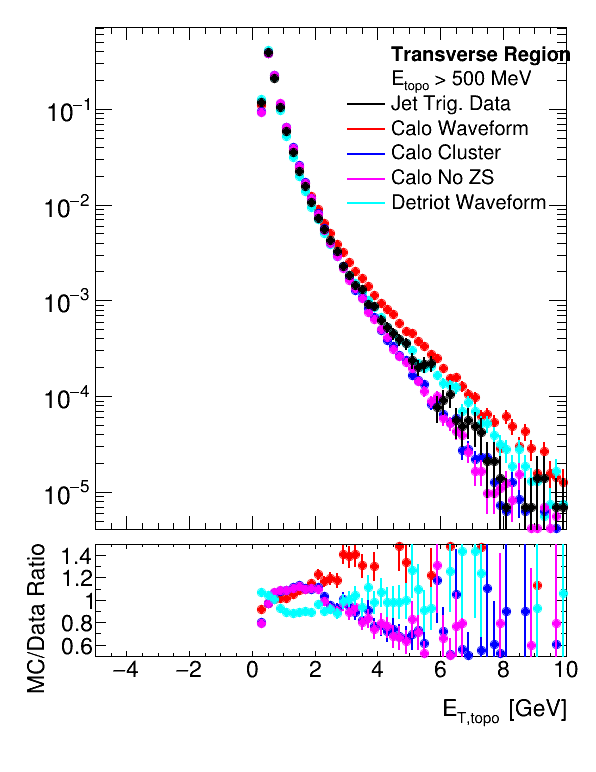
\includegraphics[width=0.32\linewidth]{Figures/initial_studies/h_topo_spectra_transverse500_Topoclusters.png}
    \caption{Topocluster transverse energy spectra in the transverse region of dijet events for various $E_{topo}$ thresholds using ana430p007 data, Run 15 calo waveform, nozero and cluster, and Run 150 (Detroit) waveform jet 10 datasets.}
    \label{fig:topo_spectra_transverse}
\end{figure}

\begin{figure}
    \centering
    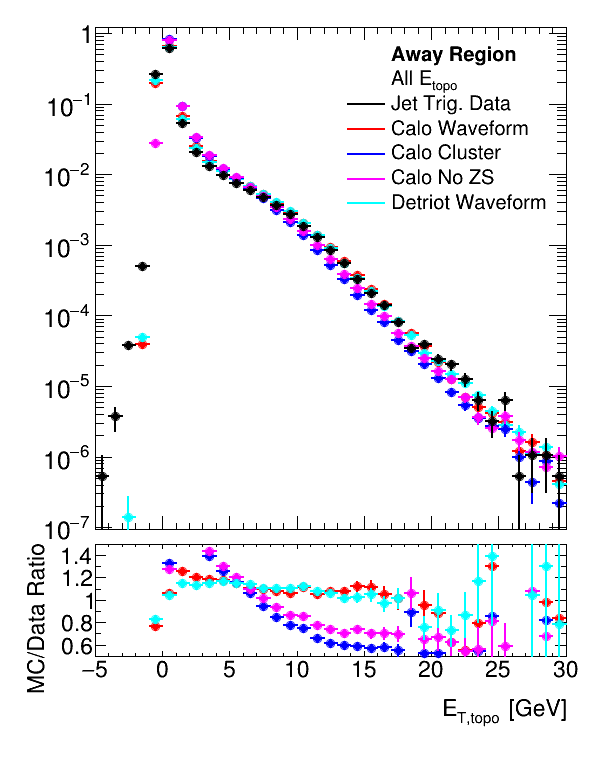
\includegraphics[width=0.32\linewidth]{Figures/initial_studies/h_topo_spectra_away-9999_Topoclusters.png}
    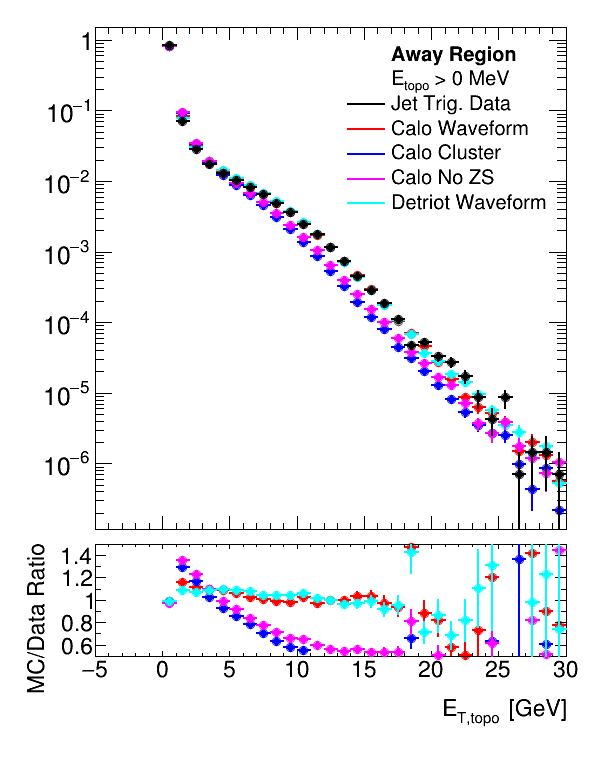
\includegraphics[width=0.32\linewidth]{Figures/initial_studies/h_topo_spectra_away0_Topoclusters.png}
    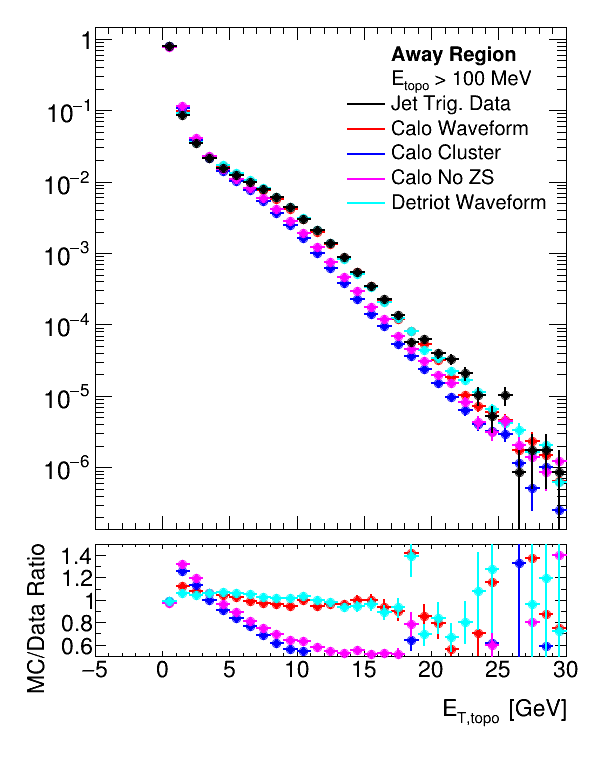
\includegraphics[width=0.32\linewidth]{Figures/initial_studies/h_topo_spectra_away100_Topoclusters.png}
    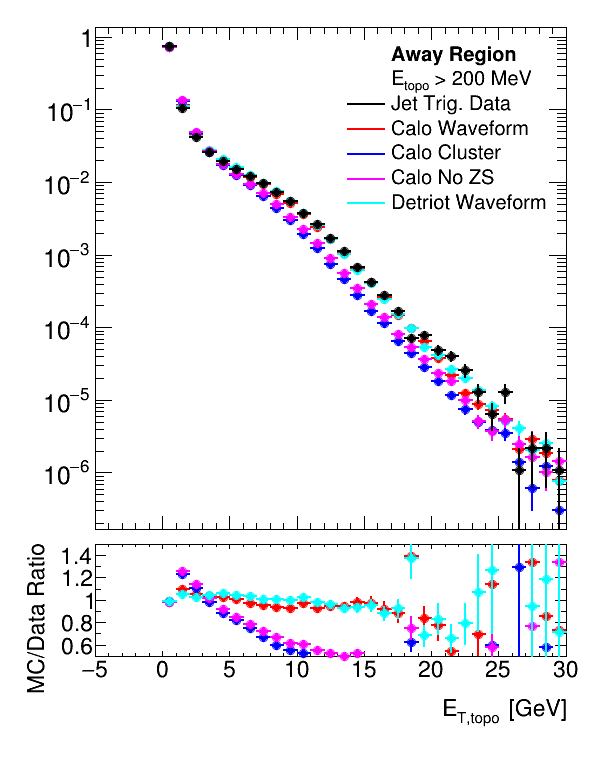
\includegraphics[width=0.32\linewidth]{Figures/initial_studies/h_topo_spectra_away200_Topoclusters.png}
    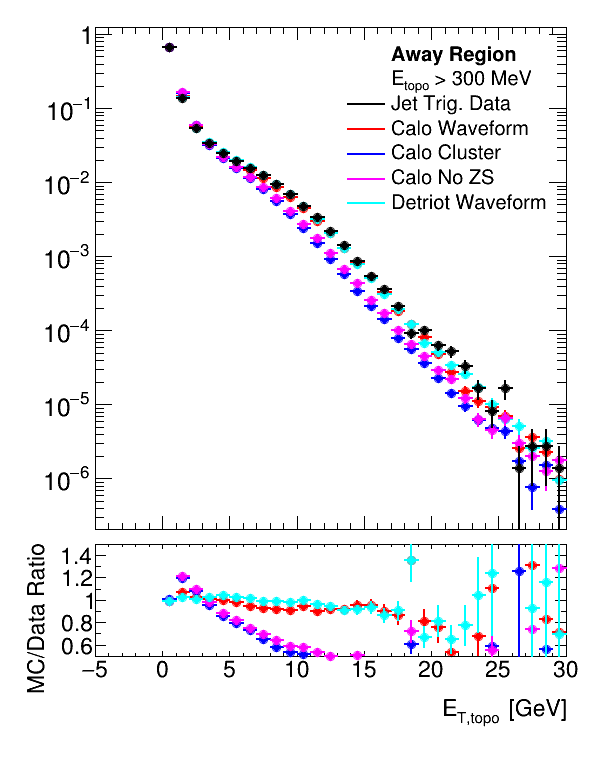
\includegraphics[width=0.32\linewidth]{Figures/initial_studies/h_topo_spectra_away300_Topoclusters.png}
    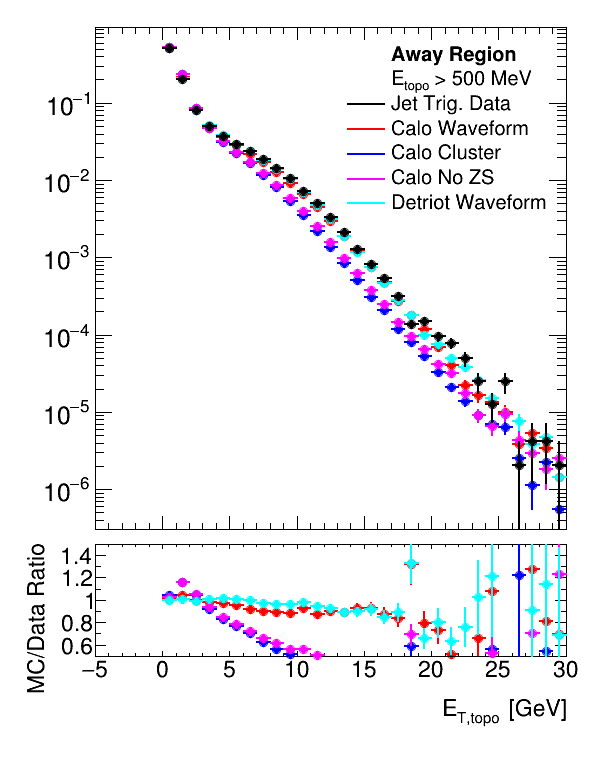
\includegraphics[width=0.32\linewidth]{Figures/initial_studies/h_topo_spectra_away500_Topoclusters.png}
    \caption{Topocluster transverse energy spectra in the away region of dijet events for various $E_{topo}$ thresholds using ana430p007 data, Run 15 calo waveform, nozero and cluster, and Run 150 (Detroit) waveform jet 10 datasets.}
    \label{fig:topo_spectra_away}
\end{figure}